\chapterimage{bg/7}


\chapter*{Annexes}

Ces annexes vont vous présenter certains problèmes rencontrés durant mon stage et les solutions mises en \oe uvre pour y pallier d'un point de vue technique.

		\section*{Gestion des «~synonymes~» dans la base de données Inforsid}
			L'insertion des données des congrès Inforsid dans la base de données alimentant l'application web était basée sur des fichiers texte : nous disposions de deux fichiers par édition, un contenant les informations sur les membres du comité de programme et un contenant celles sur les articles présentés (titre et auteur(s)), plus un fichier contenant les villes ayant accueilli chaque édition. À partir de ces fichiers, un programme en langage C avait pour tâche de déterminer la liste des chercheurs et des villes.
			
			Le principal problème de cette méthode était que les fautes de frappe sont très difficilement repérables avant l'insertion des données dans la base. En effet, les noms de chercheurs et de villes étant dispersées dans de nombreux fichiers, il aurait été fastidieux de devoir tous les contrôler à la recherche d'éventuelles erreurs. De fait la base de données était «~polluée~» de nombreux cas de noms de villes ou de personnes «~synonymes~», tels que «~Sophia~Antipolis~» et «~Sophia-Antipolis~» ou «~Cauvet~Corine~» et «~Cauvet~Corinne~».
			
			Pour résoudre ce problème, j'ai décidé de tout d'abord créer deux tables -- une pour les noms de ville et une pour les personnes -- contenant les couples potentiels de synonymes, trouvés grâce à la fonction SQL \texttt{soundex}\footnote{Documentation officielle~: \url{http://docs.oracle.com/cd/B19306_01/server.102/b14200/functions148.htm}.}. Cette méthode retourne la représentation phonétique du paramètre passé, et permet donc de comparer des noms et prénoms ne s'écrivant pas pareil mais se prononçant de la même façon. Il faut noter que cette méthode a cependant une limite non négligeable~: elle se base sur la prononciation américaine des consonnes. Chaque terme est représenté sous la forme d'une chaîne de caractères composée d'une lettre (l'initiale du terme) et de 3 chiffres représentant les consonnes suivantes, deux consonnes ayant la même prononciation étant codées par le même chiffre\footnote{Plus d'informations à l'adresse \url{http://www.archives.gov/research/census/soundex.html}.}.
			
			 J'ai également dû prendre en compte le fait que nous ne disposions pas du prénom complet pour certains chercheurs mais seulement de l'initiale, et que nous devions donc, lorsque c'est le cas, ne comparer que la phonétique du nom de famille. Enfin j'ai traité le cas où une personne change de nom au cours de sa carrière (nous avions par exemple dans la base «~Karen~Sauvagnat~» et «~Karen~Pinel-Sauvagnat~»). Le code SQL ayant permis la création de ces tables est présenté dans l'extrait de code~\ref{cod:create}.
			
			\lstinputlisting[caption={Code SQL permettant la création des tables détectant les «~synonymes~» dans la base de données alimentant l'application web présentant Inforsid.}, label=cod:create, firstline=4, lastline=29]{code/cleanDB.sql}
			
			Après la création de ces tables l'utilisateur pouvait ainsi consulter ces couples, et supprimer les faux-positifs, grâce à l'utilitaire de visualisation des données d'une table de SQL*Developer (voir figure~\ref{fig:syn}).
			
			\begin{figure}
				\centering
				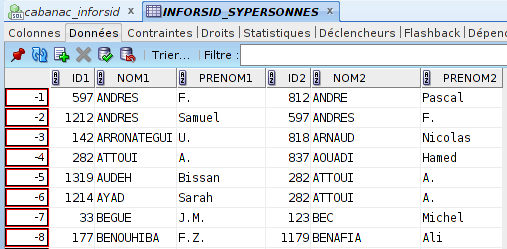
\includegraphics[width=0.8\textwidth]{annexes/syn}
				\caption{Utilitaire de visualisation des données d'une table de SQL*Developer grâce auquel l'utilisateur pouvait supprimer les couples de «~synonymes~» détectés par erreur. La table présentée ici est celle recensant les synonymes parmi les noms de chercheurs et les lignes indiquées en rouge sont des couples détectés par erreur destinés à être supprimés.}\label{fig:syn}
			\end{figure}
			
			 Après cela j'ai créé une procédure PL/SQL ayant pour but de «~fusionner~» les deux entités du couple, en modifiant les clés étrangères dans les tables les référençant et en supprimant un des deux noms. J'ai choisi de conserver le premier nom du couple, ce qui obligeait l'utilisateur à éventuellement modifier l'orthographe de celui-ci si ce n'était pas celle qui lui convenait. Le code de cette procédure est présenté dans l'extrait de code~\ref{cod:proc}.
			
			\lstinputlisting[caption={Code SQL permettant la création de la procédure ayant pour tâche de fusionner les deux entités des couples «~synonymes~» dans la base de données alimentant l'application web présentant Inforsid.}, label=cod:proc, firstline=31, lastline=65]{code/cleanDB.sql}
			 
			 La base de données était ainsi plus cohérente et la procédure facilement réutilisable. Il est cependant à noter que les fichiers CSV initiaux n'étaient pas modifiés par cette procédure, et qu'il était donc nécessaire de la relancer à chaque nouvelle insertion de données.

		 		 
			 
		\section*{Gestion des pays dans la base de données Inforsid}
			Auparavant, pour spécifier le pays correspondant aux villes destinées à être insérées dans la base de données Inforsid, il fallait parcourir le fichier contenant la liste de villes résultant du traitement des fichiers texte contenant les données de chaque édition par le programme en C. Celui-ci contenait une fonction destinée à récupérer les pays précédemment spécifiés par l'utilisateur si une liste de ville existait déjà (résultat d'un précédent traitement des données) mais cette fonctionnalité avait souvent tendance à corrompre la liste finale.
			
			J'ai alors choisi d'automatiser au maximum la procédure d'attribution d'un pays à une ville. J'ai tout d'abord créé une table référence destinée à contenir l'identifiant d'une ville, son nom et son pays dans laquelle j'ai inséré toutes les villes françaises -- téléchargées sur SQL.sh\footnote{\url{http://sql.sh/736-base-donnees-villes-francaises}}.
			
			J'ai ensuite créé une vue recensant les villes présentes dans la liste des villes concernées par le congrès Inforsid mais non présentes dans la table évoquée précédemment. Dans cette vue, l'utilisateur avait deux possibilités~:
			\begin{itemize}
				\item si des villes françaises étaient dans cette vue, c'était que leur orthographe n'était pas correcte et il devait donc les corriger (il pouvait chercher l'orthographe correcte dans la table référence),
				\item pour les villes étrangères, il modifiait leur pays et un déclencheur insérait alors ces nouvelles villes dans  la table référence (le code de ce déclencheur est présenté dans l'extrait de code~\ref{cod:trigger}).
			\end{itemize}	
			
			\lstinputlisting[caption={Code SQL permettant la création du déclencheur insérant une nouvelle ville et le pays correspondant dans la table référence dans la base de données alimentant l'application web présentant Inforsid.}, label=cod:trigger, firstline=23, lastline=33]{code/gererPays.sql}
					
			Une fois toutes les villes corrigées ou insérées dans la table référence, la vue était donc vide. L'utilisateur devait alors lancer une procédure qui mettait à jour les villes concernées par le congrès Inforsid. Le code de cette procédure est visible dans l'extrait de code~\ref{cod:pays}.
			
			\lstinputlisting[caption={Code SQL de la procédure mettant à jour les pays des villes impliquées dans le congrès Inforsid.}, label=cod:pays, firstline=37, lastline=56]{code/gererPays.sql}
			
			La détermination «~manuelle~» de l'identifiant de la nouvelle ville (\texttt{max(idV)+1}) n'est pas robuste aux accès concurrents mais étant donné que l'insertion des données n'est effectuée que par un seul utilisateur (Guillaume~Cabanac ou l'un(e) de ses stagiaires) l'utilisation d'une séquence aurait eu un intérêt minime dans notre cas.
			
			L'avantage de cette méthode est que la base de villes présentes -- et donc automatiquement gérées -- augmente d'année en année au fur et à mesure des insertions de données. Elle diffère cependant fortement de la méthode mise en place précédemment, au sens où l'attribution des pays se fait à présent après l'insertion des villes dans la base.